%!TEX root = Thesis.tex

\section{Implementation}
\label{sec:impl}

We implemented \tool{}\footnote{We plan to make MonkeyDB available open-source
soon.} to support an interface common to most storage
systems. Operations can be either key-value (KV) updates (to access data as a KV map)
or SQL queries (to access data as a relational database). \tool{} supports
transactions as well; a transaction can include multiple operations. 
Figure~\ref{fig:block_dia} shows the architecture of \tool{}. 
A client can connect to \tool{} over a TCP connection, as is
standard for SQL databases\footnote{We support the MySQL client-server
protocol using \url{https://github.com/jonhoo/msql-srv}.}. 
%See \url{https://dev.mysql.com/doc/internals/en/client-server-protocol.html}}. 
This
offers a plug-and-play experience when using
standard frameworks such as JDBC \cite{jdbc}. 
Client applications can also use \tool{} as a library in order to directly invoke the storage APIs,
or interact with it via HTTP requests, with JSON payloads.  

%The KV interface is implemented in C++.
%The SQL interface is implemented in Rust and it supports a subset of the
%standard SQL operators. For instance, it currently does not 
%support nested queries or join operators; these can be added with more
%engineering effort in the SQL-To-KV compiler. 

MonkeyDB contains a SQL-To-KV compiler that parses an input query\footnote{We
use \url{https://github.com/ballista-compute/sqlparser-rs}}, builds
its Abstract Syntax Tree (AST) and then applies the rewriting steps described in Section~\ref{sec:SQL-to-KV} 
to produce an equivalent sequence of KV API calls ({\tt read()} and {\tt write()}).
It uses a hashing routine ({\tt hash}) to generate unique keys corresponding to each cell in a table.
For instance, in order to insert a value $v$ for a column $c$ in a particular row with primary key value $\pkeyVal$, of a table $\tab$, 
we invoke {\tt write(hash($\tab$, $\pkeyVal$, $c$), $v$)}. 
We currently support only a subset of the standard SQL operators. For instance, 
nested queries or join operators are unsupported; these can be added in the
future with more engineering effort.

MonkeyDB schedules transactions from different sessions
one after the other using a single global lock.
Internally, it maintains execution state as a history consisting of a set of transaction logs, 
write-read relations and a partial session order (as discussed in \sectref{ax-kv}).
%The KV APIs {\tt read()} and {\tt write()} use the history to implement the
%operational semantics of \sectref{op-kv}.
%The function {\tt write()} simply records the operation in the transaction log of the history. 
On a {\tt read()}, MonkeyDB first collects a set of possible writes present in transaction log 
that can potentially form write-read (read-from) relationships, and then 
invokes the consistency checker (Figure~\ref{fig:block_dia}) to confirm
validity under the chosen isolation level.
Finally, it randomly returns one of the values associated with valid writes.
A user can optionally instruct MonkeyDB to only select
from the set of \textit{latest} valid write per session. This option helps limit weak behaviors
for certain reads.


The implementation of our consistency checker is based on prior work
\cite{DBLP:journals/pacmpl/BiswasE19}. It maintains 
the write-read relation as a graph, and detects cycles (isolation-level
violations) using DFS traversals on the graph. The consistency checker is an independent 
and pluggable module: we have one for Read Committed and one for Causal
Consistency, and more can be added in the future.



%A user can optionally instruct  to only choose 
%turn off weak reads for a particular
%transaction. In this case, each read of that transaction will choose the latest valid write. This
%mode is useful when evaluating assertions.

%can be We allow the non-determinism in {\tt read()}, in choosing the return value, to
%be resolved with different strategies.    
%The default strategy is uniform-at-random, but one can instead do: (1)
%weakest-read or (2) strongest-read, or (3) weak-biased-read.  
%Weakest-read strategy always returns a value corresponding to the oldest valid write.    
%Strongest-read strategy always returns a value corresponding to the latest valid
%write (useful when evaluating assertions). 
%Weak-biased-read strategy chooses an older write with a higher probability than
%a later write. 
%We discuss the effect of these strategies in \sectref{oltp}.

\begin{figure}
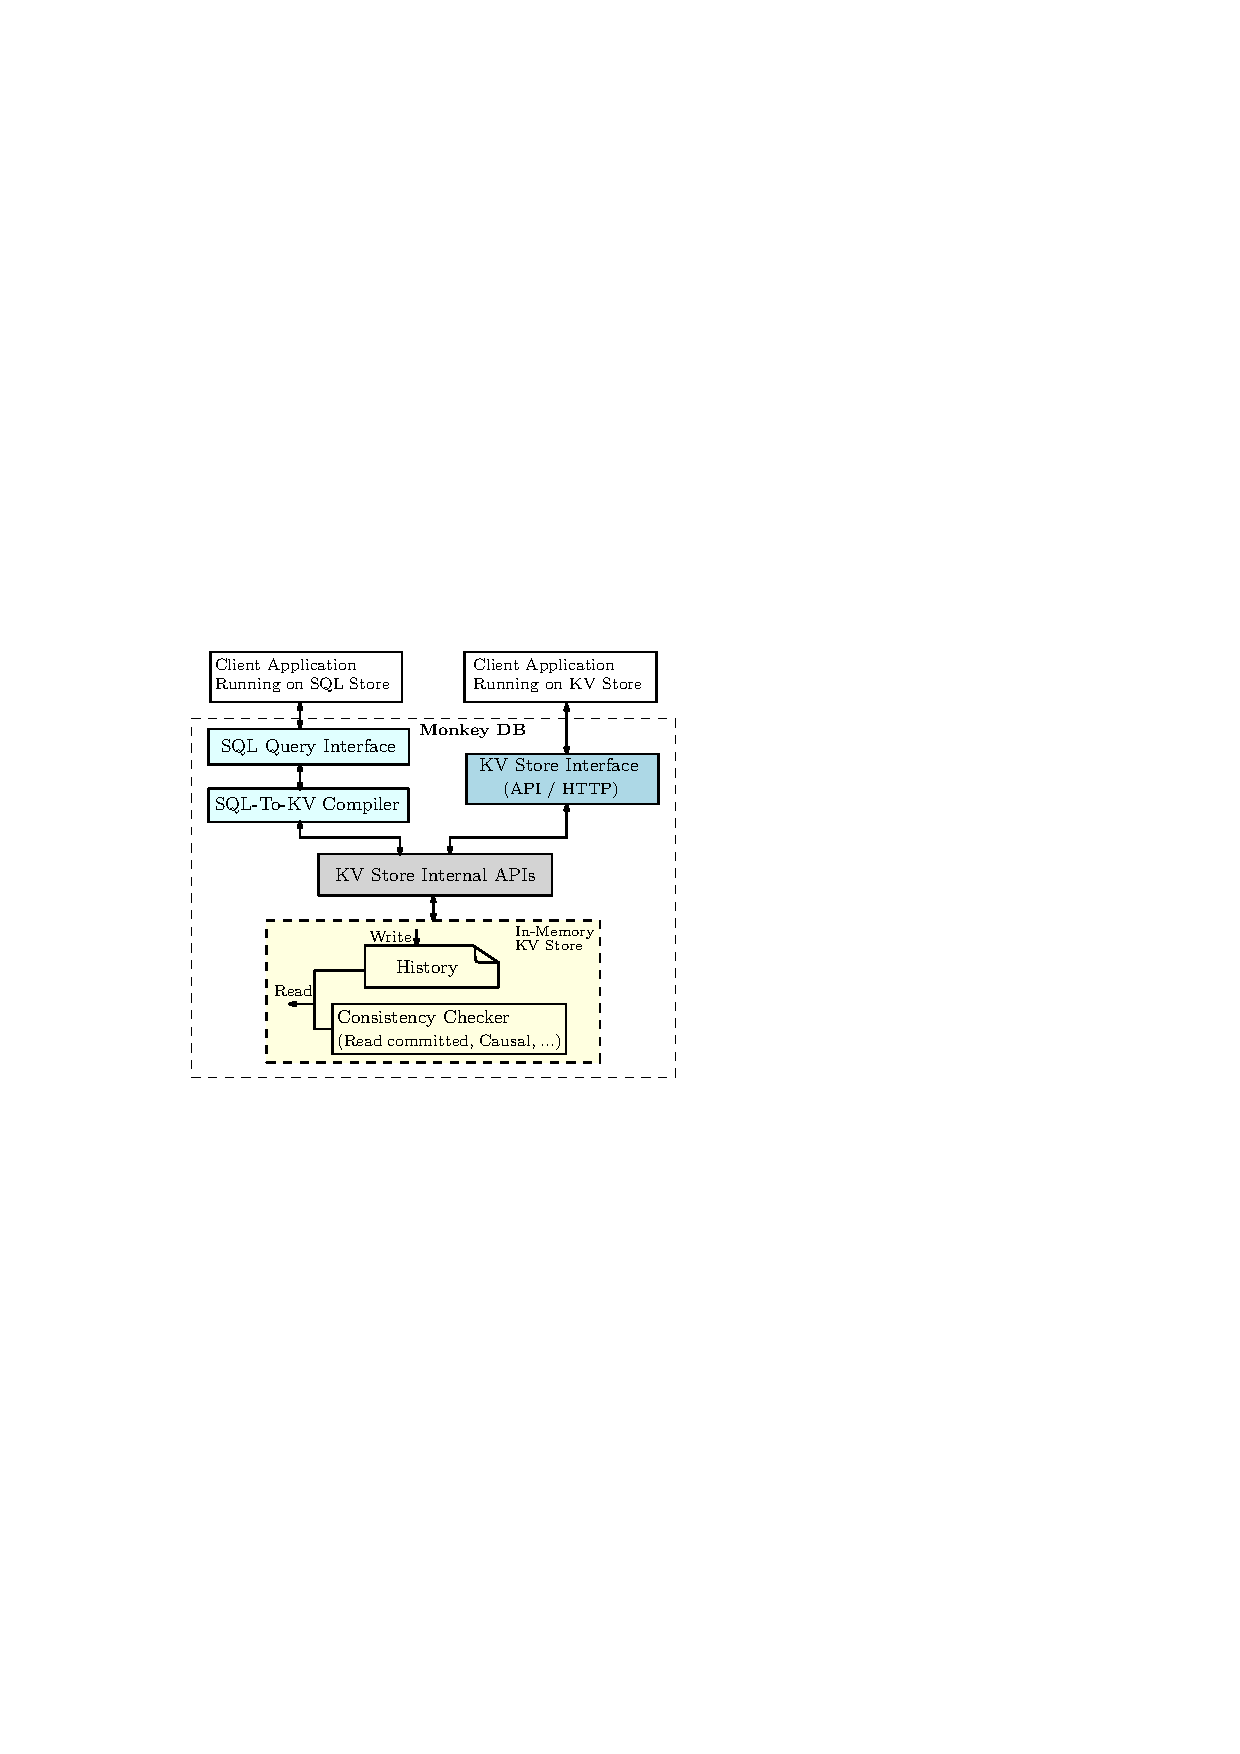
\includegraphics[scale=0.8]{Sources/sql/figures/block_dia.pdf}
\caption{Architecture of \tool{}}
\label{fig:block_dia}
\end{figure}

%The next two sections present an evaluation of \tool{} on a set of
%micro-benchmarks used in prior papers (\sectref{micro}) as well as applications
%from the OLTP benchmark suite \cite{difallah2013oltp} that consists of
%representative transaction processing workloads running on SQL databases
%(\sectref{oltp}).
%We measure the effectiveness of \tool{} using the \textit{coverage} of weak
%behaviors as well as the ability to break invalid assertions.

%in exploring weak behaviors and in detecting invariant violations on various real-world applications. 
%For this purpose, we used \tool{} in place of actual storage systems and carried out experiments on two sets of benchmarks:
%(1)~a set of microbenchmarks containing shopping cart~\cite{sivaramakrishnan2015declarative}, Twitter~\cite{twissandra}, stack~\cite{cavNagarMJ20} and courseware~\cite{DBLP:conf/esop/NairP020} applications that are representative of real-world services running on Key-Value stores,  
%(2)~a set of applications from OLTP-Bench (Online Transaction Processing) benchmark suite~\cite{difallah2013oltp} that are representative of transaction processing workloads running on SQL-based relational databases.
%We test these two sets of applications on Key-Value and SQL store interfaces of \tool{} respectively.
%We now discuss our experiments and observed results in detail in Section~\ref{ss:micro} and Section~\ref{sec:oltp}.


